\documentclass[tikz,border=6pt]{standalone}
\usepackage[T1]{fontenc}
\usepackage[utf8]{inputenc}
\usepackage{helvet}
\renewcommand{\familydefault}{\sfdefault}
\usepackage{xcolor}
\usetikzlibrary{arrows.meta}
\definecolor{cblue}{HTML}{1F4E79}
\definecolor{cgreen}{HTML}{2E7D32}
\definecolor{cred}{HTML}{C62828}
\definecolor{cgrey}{HTML}{808080}
\definecolor{paleblue}{HTML}{E8F0F8}
\definecolor{palegreen}{HTML}{E8F5E9}
\definecolor{palered}{HTML}{FFEBEE}
\definecolor{palegrey}{HTML}{F5F5F5}
\begin{document}

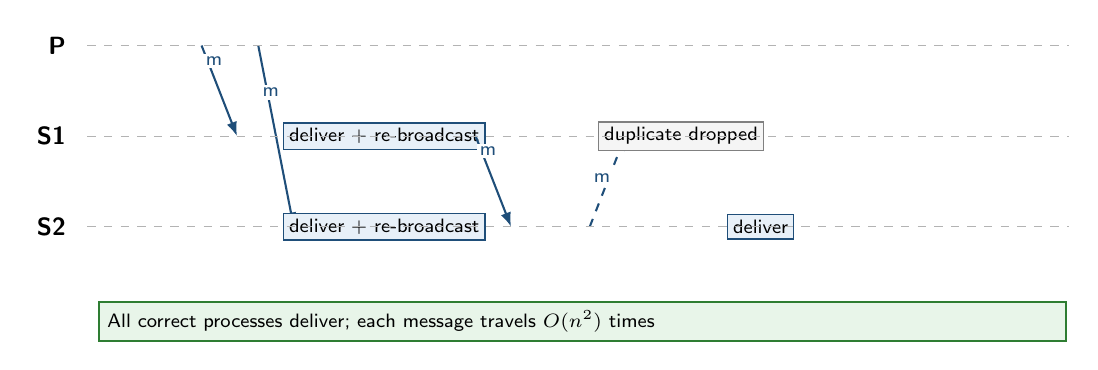
\begin{tikzpicture}[x=1cm,y=1cm]
\draw[-{Latex[length=1.8mm]},cblue,solid,line width=0.75pt] (1.45,0.000) -- (1.90,-1.150) node[pos=0.35,above,yshift=3pt,fill=white,inner sep=1pt,font=\scriptsize] {m};
\draw[-{Latex[length=1.8mm]},cblue,solid,line width=0.75pt] (2.17,0.000) -- (2.62,-2.300) node[pos=0.35,above,yshift=3pt,fill=white,inner sep=1pt,font=\scriptsize] {m};
\node[draw=cblue,fill=paleblue,line width=0.5pt,inner sep=2pt,font=\scriptsize,align=center] at (3.77,-1.150) {deliver + re-broadcast};
\draw[-{Latex[length=1.8mm]},cblue,solid,line width=0.75pt] (4.93,-1.150) -- (5.38,-2.300) node[pos=0.35,above,yshift=3pt,fill=white,inner sep=1pt,font=\scriptsize] {m};
\node[draw=cblue,fill=paleblue,line width=0.5pt,inner sep=2pt,font=\scriptsize,align=center] at (3.77,-2.300) {deliver + re-broadcast};
\draw[-{Latex[length=1.8mm]},cblue,dashed,line width=0.75pt] (6.38,-2.300) -- (6.83,-1.150) node[pos=0.35,above,yshift=3pt,fill=white,inner sep=1pt,font=\scriptsize] {m};
\node[draw=cgrey,fill=palegrey,line width=0.5pt,inner sep=2pt,font=\scriptsize,align=center] at (7.54,-1.150) {duplicate dropped};
\node[draw=cblue,fill=paleblue,line width=0.5pt,inner sep=2pt,font=\scriptsize,align=center] at (8.55,-2.300) {deliver};
\node[anchor=north west,draw=cgreen,fill=palegreen,line width=0.5pt,inner sep=3pt,text width=12.069999999999999cm,align=left,font=\scriptsize] at (0.14,-3.250) {All correct processes deliver; each message travels $O(n^2)$ times};
\draw[cgrey!60,line width=0.4pt,dashed] (0,0.000) -- (12.469999999999999,0.000);
\node[anchor=east,font=\small\bfseries] at (-0.15,0.000) {P};
\draw[cgrey!60,line width=0.4pt,dashed] (0,-1.150) -- (12.469999999999999,-1.150);
\node[anchor=east,font=\small\bfseries] at (-0.15,-1.150) {S1};
\draw[cgrey!60,line width=0.4pt,dashed] (0,-2.300) -- (12.469999999999999,-2.300);
\node[anchor=east,font=\small\bfseries] at (-0.15,-2.300) {S2};
\end{tikzpicture}
\end{document}
